\documentclass[border=6pt]{standalone}
\usepackage[T1]{fontenc}
\usepackage{courier}
\usepackage[scaled=0.95]{helvet}
\renewcommand{\familydefault}{\sfdefault}
\usepackage{sfmath}
\usepackage[version=4]{mhchem}
\usepackage{tikz}
\usepackage{pgfplots}
\pgfplotsset{compat=newest}
\usetikzlibrary{arrows.meta,positioning,calc,fit,backgrounds,shapes.geometric,decorations.pathreplacing,patterns}
\definecolor{ink}{HTML}{17233A}
\definecolor{inksoft}{HTML}{44506A}
\definecolor{teal}{HTML}{0E6B6B}
\definecolor{tealsoft}{HTML}{E5F0EF}
\definecolor{amber}{HTML}{B26B12}
\definecolor{ambersoft}{HTML}{FBF0DF}
\definecolor{blue}{HTML}{2F6690}
\definecolor{bluesoft}{HTML}{E3ECF4}
\definecolor{plum}{HTML}{7A4D8C}
\definecolor{plumsoft}{HTML}{EFE7F3}
\definecolor{greyc}{HTML}{8A94A3}
\definecolor{linec}{HTML}{D3DCE1}
\definecolor{oxy}{HTML}{C0392B}
\definecolor{carb}{HTML}{3B4252}
\definecolor{hyd}{HTML}{E6E9EE}
\definecolor{nit}{HTML}{2F6690}
\tikzset{
  every picture/.style={line cap=round,line join=round},
  lab/.style={font=\small, text=inksoft},
  >={Stealth[length=7pt]},
}
\pgfplotsset{
  every axis/.append style={axis line style={inksoft}, tick style={inksoft}, tick label style={font=\footnotesize, text=inksoft}, label style={font=\small, text=ink}},
}
% fragment tile: \frag{node name}{position}{colour}{content}
\newcommand{\frag}[4]{\node[draw=#3, fill=#3!12, line width=1.4pt, rounded corners=6pt, minimum width=1.25cm, minimum height=1.05cm, text=#3, font=\bfseries] (#1) at (#2) {#4};}
\newcommand{\ring}{\tikz[baseline=-0.6ex]{\draw[line width=1.1pt] (0:0.3)--(60:0.3)--(120:0.3)--(180:0.3)--(240:0.3)--(300:0.3)--cycle; \draw[line width=0.8pt] (0,0) circle (0.16);}}
\newcommand{\bond}[2]{\draw[ink, line width=2.2pt] (#1) -- (#2);}

\begin{document}
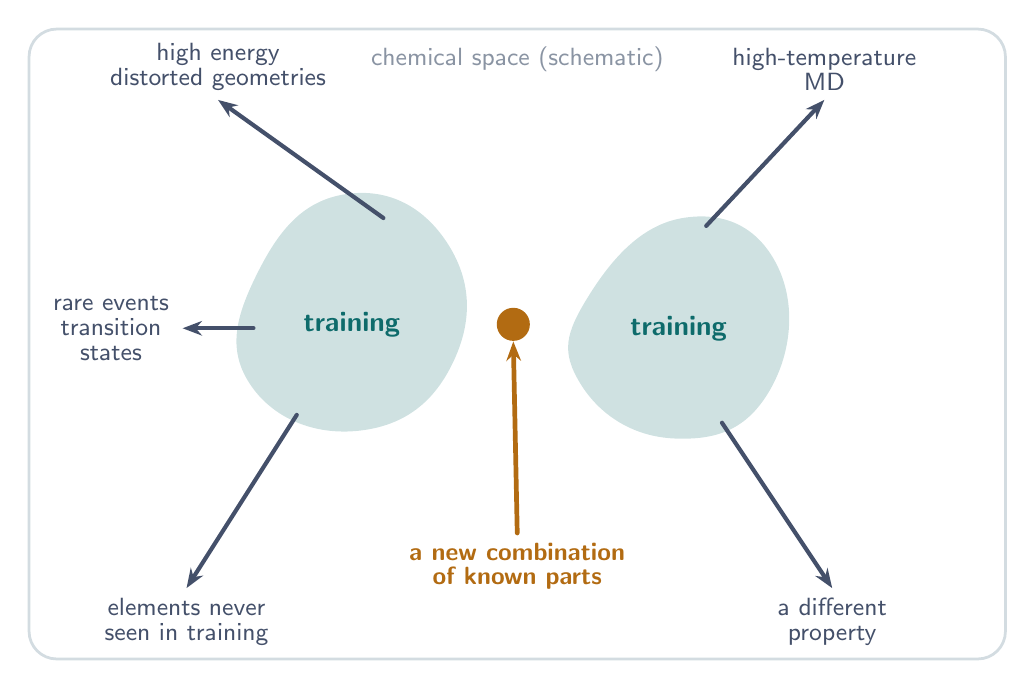
\begin{tikzpicture}
\draw[linec, line width=1pt, rounded corners=10pt] (-6.2,-4.0) rectangle (6.2,4.0);
\node[font=\small, text=greyc, anchor=north] at (0,3.9) {chemical space (schematic)};
\fill[teal, fill opacity=0.2] plot[smooth cycle, tension=0.8] coordinates {(-3.3,0.9) (-2.2,1.9) (-0.9,1.3) (-0.8,-0.2) (-2.0,-1.1) (-3.4,-0.5)};
\fill[teal, fill opacity=0.2] plot[smooth cycle, tension=0.8] coordinates {(0.9,0.6) (2.1,1.6) (3.3,1.0) (3.2,-0.6) (2.0,-1.2) (0.8,-0.5)};
\node[font=\bfseries, text=teal] at (-2.1,0.25) {training};
\node[font=\bfseries, text=teal] at (2.05,0.2) {training};
\foreach \x/\y/\lx/\ly/\t/\a in {-1.7/1.6/-3.8/3.1/high energy\\[-2pt]distorted geometries/south, 2.4/1.5/3.9/3.1/high-temperature\\[-2pt]MD/south, -2.8/-0.9/-4.2/-3.1/elements never\\[-2pt]seen in training/north, 2.6/-1.0/4.0/-3.1/a different\\[-2pt]property/north}{
  \draw[->, inksoft, line width=1.5pt] (\x,\y) -- (\lx,\ly);
  \node[font=\small, text=inksoft, align=center, anchor=\a] at (\lx,\ly) {\t};
}
\draw[->, inksoft, line width=1.5pt] (-3.35,0.2) -- (-4.25,0.2);
\node[font=\small, text=inksoft, align=center, anchor=east] at (-4.3,0.2) {rare events\\[-2pt]transition\\[-2pt]states};
\node[circle, fill=amber, minimum size=0.42cm, inner sep=0] (n) at (-0.05,0.25) {};
\draw[->, amber, line width=1.7pt] (0.0,-2.4) -- (n.south);
\node[font=\small\bfseries, text=amber, align=center, anchor=north] at (0.0,-2.4) {a new combination\\[-2pt]of known parts};
\end{tikzpicture}
\end{document}
